\section{スパース性}
第5章では$\ell$1制限のもとでは解がスパースになることを学習した。しかし、サポートベクターマシンにおいては双対解$\bm{\hat{\alpha}}$は$\ell$1制限がなくともスパースになる傾向があることを解説する。

$\min_{\bm{w}, \gamma, \xi}\max_{\alpha, \beta}{\it{L}}(\bm{w}, \gamma, \bm{\xi}, \bm{\alpha}, \bm{\beta})\text{\ \ \ }s.t.\text{\ \ \ }\bm{\alpha} \ge \bm{0}, \bm{\beta} \ge \bm{0}$
はKKT最適性条件を満たすので、
\begin{eqnarray}
  \alpha_i(m_i - 1 + \xi_i) = 0 \\
  \beta_i\xi_i = 0 
\end{eqnarray}
これに$\bm{\alpha} + \bm{\beta} = \bm{C}$を代入すると、以下の結果が得られる。
\begin{eqnarray}
  \alpha_i = 0 \Longleftrightarrow m_i > 1 \\
  \label{margin}
  0 < \alpha_i < C \Longleftrightarrow m_i = 1 \\
  \alpha_i = C \Longleftrightarrow m_i < 1 
\end{eqnarray}

\begin{figure}[h]
  \centering
  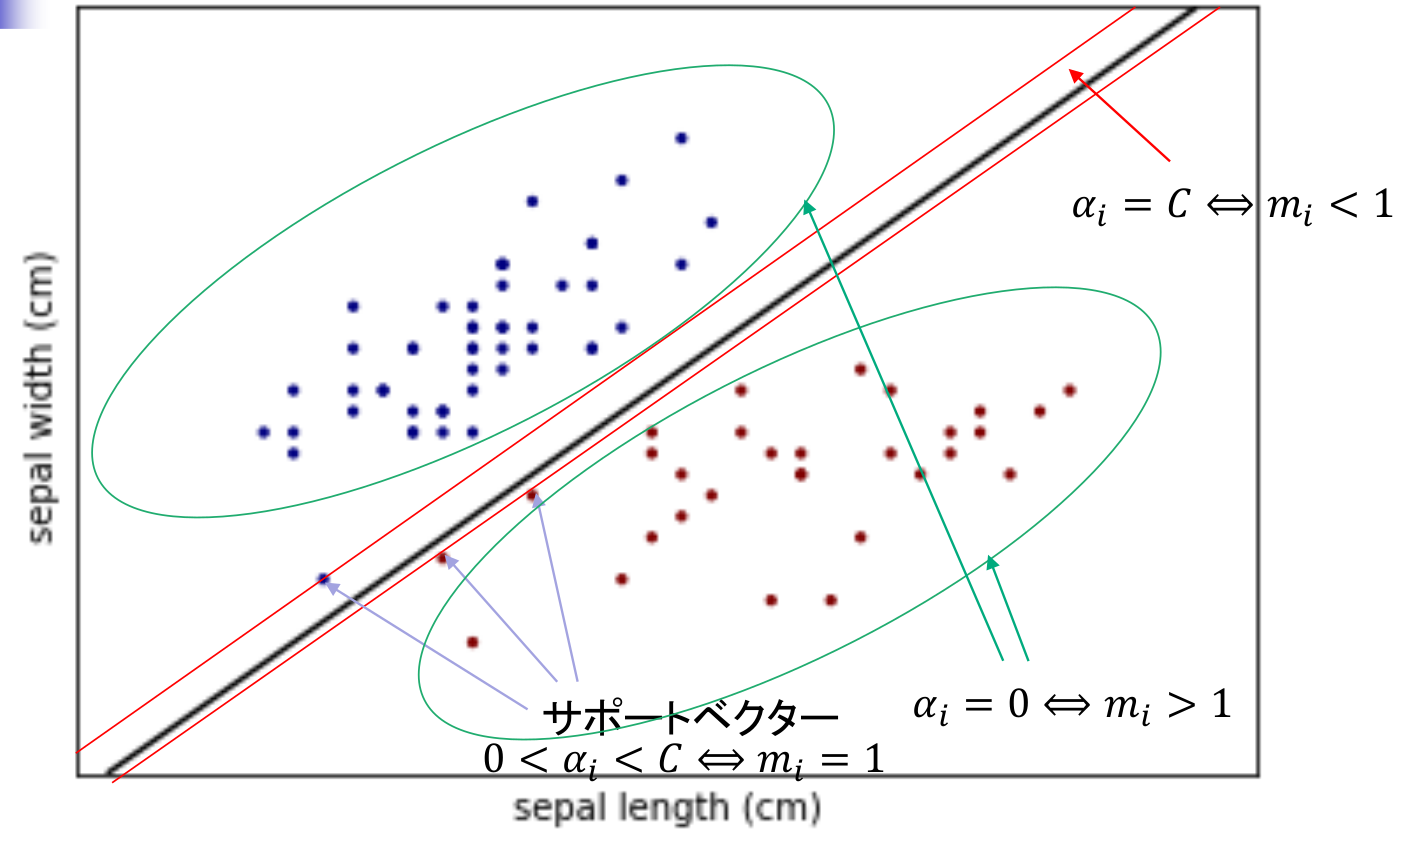
\includegraphics[width=5cm]{figure/section3/figure1.png}
  \caption{$m_i$と$\alpha_i$の関係}
\end{figure}

特に、式\ref{margin}の条件におけるサンプルを「サポートベクトル」と呼ぶ。このとき、$m_i = (\bm{w}^{\mathrm{T}}\bm{x_i} + \gamma)y_i = 1$となるので、
\begin{eqnarray}
  \begin{split}
    \hat{\gamma} = \frac{1}{y_i} - \hat{\bm{w}}^{\mathrm{T}}\bm{x_i} \\
    $= y_i - \hat{\bm{w}}^{\mathrm{T}}\bm{x_i} \\
    $= y_i - \sum_{j=1}^{n}\hat{\alpha_j}y_j\bm{x_j}\bm{x_i} \\
    $= y_i - \sum_{j=1}^{n}\hat{\alpha_j}y_j\bm{x_i}^{\mathrm{T}}\bm{x_j}
  \end{split}
\end{eqnarray}
となり、切片$\hat{\gamma}$を求めることができる。


